\documentclass[9pt,twocolumn,twoside]{../../styles/osajnl}
\usepackage{fancyvrb}
\journal{i524} 

\title{Real-time Visualization of Happiness Quotient across English regions based on Twitter data}

\author[1,*]{Sowmya Ravi}
\author[2]{Sriram Sitharaman}
\author[3]{Shahidhya Ramachandran}

\affil[1]{School of Informatics and Computing, Bloomington, IN 47408, U.S.A.}
\affil[2]{School of Informatics and Computing, Bloomington, IN 47408, U.S.A.}
\affil[3]{School of Informatics and Computing, Bloomington, IN 47408, U.S.A.}

\affil[*]{Corresponding authors: sowravi@iu.edu, srirsith@iu.edu, shahrama@iu.edu}

\dates{project-001, \today}

\ociscodes{Real-time streaming, data visualization, Twitter, Natural Language Processing}

% replace this with your url in github/gitlab
\doi{\url{https://github.com/cloudmesh/sp17-i524/tree/master/project/S17-IR-P001/report/report.pdf}}


\begin{abstract}
This project involves development of a real-time system which streams live data from twitter to visualize the "Happiness index" across the English-speaking regions in the world. Live data from twitter is injected into the system using streaming API in spark. All possible tweets are taken into consideration for analyzing the overall happiness level of people tweeting from different locations. Suitable classifier will be built to identify if the tweet is positively biased. The results of the Language processing algorithm will be visualized in  real-time using d3.js.
\end{abstract}

\setboolean{displaycopyright}{true}

\begin{document}

\flushbottom % Makes all text pages the same height

\maketitle % Print the title and abstract box

\tableofcontents % Print the contents section
\maketitle

\section{Introduction}
In 1969, Drs. Jerry Boucher and Charles E. Osgood, psychologists at the University of Illinois, proposed the 'Pollyanna Hypothesis' which asserts that "there is a universal human tendency to use evaluatively positive words more frequently and diversely than evaluatively negative words in communicating" \cite{BOUCHER19691}. Such theories were hard to validate due to the absence of significant data and the lack of generality. With Social media turning into the primary platform where people express on a day-to-day basis these claims can be analysed by sampling a portion of the data and applying Natural Language Processing algorithms to determine positivity/negativity of this data. The first step in this process involves extraction of data from Social media using the corresponding APIs. Once the data has been extracted, it is cleaned and restructured to make it suitable for analysis. The results of the Analysis are then visualized in a dashboard to better understand the outcomes.\\
Microblogging website like Twitter is used for analysing behaviour of people because it has emerged to be one of the predominant platforms where people express their opinions about current issues, complain about products, discuss details of on-going events etc. Twitter data also aids in understanding behavioral patterns across diverse demographics - location, gender etc. Twitter generates nearly 200,000 tweets in less than a minute. This large sample can then be used to test the hypothesis. Big data technologies prove to be particularly useful in storing, processing and analysing such large data sets. It also makes it possible to setup real-time systems that can output results with a latency of very few seconds. \\
This project involves extraction of Twitter data using it's API through Python. This data is stored and manipulated in Cassandra which is then fed to Kafka. Kafka streamlines this data for analysis in Spark which is finally visualized using D3.js. 

\section{Execution Summary}
The approximate schedule for completion of this project has been outlines in the section below:
\begin{enumerate}
\item {Mar 6 - Mar 12, 2017} Create virtual machines on Chameleon, FutureSystems and Jetstream clouds using Cloudmesh and submit the project proposal.
\item {Mar 13-Mar 19, 2017} Deploy Hadoop cluster to the clouds using Cloudmesh and create Ansible playbook to install the required software packages (Cassandra,D3.js,Kafka etc.) to the clusters  and to upload the twitter data.
\item {Mar 20-Mar 26, 2017} Pre-processing of the tweets to create required features for using in the Natural Language Processing algorithm. Building a language model to estimate the Happiness quotient
\item {Mar 27-Apr 02, 2017} Develop an interactive visualization of the analysed data in D3.js
\item {Apr 03-Apr 09, 2017} Continuing with the D3.Js visualization and connecting with streaming data from twitter to convert it into a live dashboard.
\item {Apr 10 - Apr 16, 2017} Create software package that can be readily deployed in Python
\item {Apr 17-Apr 23, 2017} Complete the partially done  Project Report
\end{enumerate}

\section{System Architecture}
The streaming pipeline for analysing the data consists of different components to aid in different stages of the analysis. The architecture of these components have been elaborated in this section.
\subsection{Cassandra}
\subsection{Apache Kafka}
Apcha Kafka is used as the queuing system for sending pulses of data to Pyspark. The tweets are pushed from Cassandra/Python to Kafka as and when the tweet is generated with a latency of less than a second. Kafka system is coordinated by three main components- Producer, Consumer and broker. Producer produces the data over topics, Brokers control the workload alloccated to the consumers and the consumers process the data. 
\section{Workflow}
The project will make use of the following four components. 
\begin{enumerate}
    \item Apache Spark
    \item Apache Kafka
    \item Apache Cassandra
    \item D3.js
\end{enumerate}

The Architecture of the system is shown in Fig.1
\begin{figure}[htbp]
\centering
\fbox{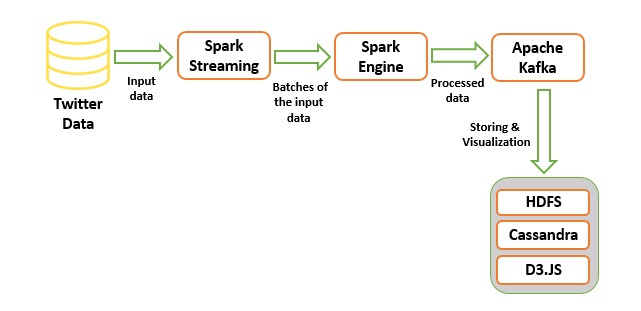
\includegraphics[width=\linewidth]{images/spark}}
\caption{Architecture}
\label{fig:false-color}
\end{figure}
\subsection{Python}
Python is used as the platform for collecting real-time data from Twitter. Using the 'tweepy' package, a tweet extracting module was built which authenticates the collection of data from Twitter's API. This is done by using the 'Consumer key' and an 'Access token' generated by Twitter's developer API. Tweets get collected at the rate of generation as a json object. This data is then parsed to extract date, textual content and location which can then be stored in Cassandra.
\subsection{Phase 1: Streaming Twitter data using Apache Spark}
Spark is a high speed in-memory data engine which is specialized to perform tasks such as streaming or requiring repeated access to datasets. The objective is to obtain the happiness index of tweets from different English speaking countries around the world. Thus it will require a fairly large amount of tweets collected over a time frame(TBD). Spark's framework provides the facility to work with a variety of data formats including text. Spark streaming which is the extension of the core spark API aids in the streaming process and delivers it to the core engine. The data is then passed to Apache Kafka which helps in pipeline processing
\subsection{Phase 2: Kafka}
Kafka, a queueing system serves as an ingestion backbone to Apache spark. It is a super-fast, low-latency, distributed and partitioned stream processing service. Kafka being highly reliable and scalable, is perfect for integrating the huge stream of twitter data to a data sink. 

\subsection{Phase 3: Apache Cassandra}
Cassandra was chosen as the database because of it's high scalability and reliability. Cassandra used along with spark streaming and kafka forms an excellent base for real time analytics. Cassandra being a NoSQL database is well suited to store unstructured textual data. A feature that makes Cassandra stand out is that it is a column oriented database which makes it horizontally scalable too. 

\subsection{Phase 4: D3.js}

Real time visualization of the processed data streamed from Kafka message queuing service would be created to view the results from the analytics performed on the twitter data.


\section{Conclusion}

Put in some conclusion based on what you have researched

\paragraph{Acknowledgement}

Put in the information for this class and who may sponsor
you. Examples will be given later
\bibliography{references}
\end{document}
